\section{The points}

I made a distinction between the point used in Euclidean geometry and the point
used to represent an element of a statistical cloud. In the first case, I use as
object a \tkzname{node}, which means that the representation of the point cannot
be modified by a \tkzname{scale}; in the second case, I use as object a
\tkzname{plot mark}. The latter can be scaled and have more varied forms than
the node.

The new macro is \tkzNameMacro{tkzDefPoint}, it allows to use \TIKZ-specific
options as a shift and the values are processed with tkz-base. Moreover, if
calculations are needed then the \tkzNamePack{xfp} package takes care of them.
You can use Cartesian or polar coordinates.

\subsection{Defining a point in Cartesian coordinates: \tkzcname{tkzDefPoint}}
\hypertarget{tdp}{}

\begin{NewMacroBox}{tkzDefPoint}{\oarg{local options}\parg{x,y}\var{name} or \parg{a:r}\var{name}}%
\begin{tabular}{lll}%
arguments &  default & definition  \\
\midrule
\TAline{x,y}{no default}{$x$ and $y$ are two dimensions, by default in cm.}
\TAline{a:r}{no default}{$a$ is an angle in degrees, $r$ is a dimension}
\bottomrule
\end{tabular}

\medskip
\noindent{The mandatory arguments of this macro are two dimensions expressed
with decimals, in the first case they are two measures of length, in the second
case they are a measure of length and the measure of an angle in degrees}.

\medskip
\begin{tabular}{lll}%
\toprule
options             & default & definition   \\
\midrule
\TOline{shift} {(0,0)} {value spacing}
 \bottomrule
\end{tabular}

\medskip
\noindent{All the options of \TIKZ\ that we can apply to \tkzname{coordinate},
are applicable (well I hope!) as for example the option \tkzname{label} defined
with the library \tkzname{quotes}.}
\end{NewMacroBox}

\subsubsection{Use of \tkzname{shift}}

\tkzname{shift} allows the points to be placed in relation to each other.

\begin{tkzexample}[latex=8cm,small]
\begin{tikzpicture}[trim left=-1cm]
  \tkzDefPoint(2,3){A}
  \tkzDefPoint[shift={(2,3)}](31:3){B}
  \tkzDefPoint[shift={(2,3)}](158:3){C}
  \tkzDrawSegments[color=red,
                   line width=1pt](A,B A,C)
  \tkzDrawPoints[color=red](A,B,C)
\end{tikzpicture}
\end{tkzexample}

\subsection{Placing a label with the library \tkzname{quotes}}

I prefer not to mix operations and use \tkzcname{tkzLabelPoint} to place labels.
See the section \enquote{The  Quotes Syntax} in the \TIKZ\ manual.

\begin{tkzexample}[latex=7cm,small]
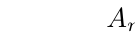
\begin{tikzpicture}[trim left=-1cm]
  \tkzDefPoint["-60:$A_n$" ](2,3){A}
  \tkzDefPoint[shift={(2,3)},%
     "$B_n$" above left](31:3){B}
  \tkzDefPoint[shift={(2,3)},%
     "$C_n$" above right](158:3){C}
  \tkzDrawSegments[color=red,%
         line width=1pt](A,B A,C)
  \tkzDrawPoints[color=red](A,B,C)
\end{tikzpicture}
\end{tkzexample}


\subsubsection{Rotation with \tkzname{shift} and \tkzname{scope}}

Preferable to rotate is to use a \tkzNameEnv{scope} environment.

\begin{tkzexample}[latex=7cm,small]
\begin{tikzpicture}[scale=.75,rotate=90]
  \tkzDefPoint[label=right:$A_n$](2,3){A}
  \begin{scope}[shift={(A)}]
     \tkzDefPoint[label= right:$B_n$](31:3){B}
     \tkzDefPoint[label= right:$C_n$](158:3){C}
  \end{scope}
  \tkzDrawSegments[color=red,%
           line width=1pt](A,B A,C)
  \tkzDrawPoints[color=red](A,B,C)
\end{tikzpicture}
\end{tkzexample}

\subsubsection{Forms and coordinates}

Here we must follow the syntax of \tkzNamePack{xfp}. It is always possible to go
through \tkzNamePack{pgfmath} but in this case, the coordinates must be
calculated before using the macro \tkzcname{tkzDefPoint}.

\begin{tkzexample}[latex=7cm,small]
\begin{tikzpicture}[scale=.75]
  \tkzInit[xmax=6,ymax=6]
  \tkzGrid
  \tkzSetUpPoint[shape = circle,color = red,%
                 size = 4,fill = red!30]
  \tkzDefPoint(-1+1,-1+4){O}
  \tkzDefPoint({3*ln(exp(1))},{exp(1)}){A}
  \tkzDefPoint({4*sin(pi/6)},{4*cos(pi/6)}){B}
  \tkzDefPoint({4*sin(pi/3)},{4*cos(pi/3)}){B'}
  \tkzDefPoint[shift={(1,3)}](30:3){A'}
  \tkzDrawPoints(O,A,B)
  \tkzDrawPoints[color=red,shape=cross out](B',A')
  \tkzLabelPoints(A,O,B,B',A')
\end{tikzpicture}
\end{tkzexample}

\subsubsection{Scope and \tkzcname{tkzDefPoint}}

First, we can use the \tkzNameEnv{scope} of \TIKZ.
In the following example, we have a way to define an isosceles triangle.

\begin{tkzexample}[latex=7cm,small]
\begin{tikzpicture}[scale=1]
  \begin{scope}[rotate=30]
    \tkzDefPoint(2,3){A}
    \begin{scope}[shift=(A)]
       \tkzDefPoint(90:5){B}
       \tkzDefPoint(30:5){C}
    \end{scope}
  \end{scope}
  \tkzDrawSegments[color=blue](A,B B,C C,A)
  \tkzDrawPoints(A,B,C)
  \tkzLabelPoints[above](B,C)
  \tkzLabelPoints[below](A)
\end{tikzpicture}
\end{tkzexample}
%<--------------------------------------------------------------------------->

\subsection{Definition of points in Cartesian coordinates: \tkzcname{tkzDefPoints}} \hypertarget{tdps}{}

\begin{NewMacroBox}{tkzDefPoints}{\oarg{local options}\var{$x_1/y_1/n_1,x_2/y_2/n_2$, ...}}%
$x_1$ and $y_1$ are the coordinates of a referenced point $n_1$

\begin{tabular}{lll}%
\toprule
arguments &  example  &   \\
\midrule
\TAline{$x_i/y_i/n_i$}{\tkzcname{tkzDefPoints\{0/0/O,2/2/A\}}}{}
\end{tabular}
\end{NewMacroBox}

\subsubsection{Definition of points}

\begin{tkzexample}[latex=6cm,small]
\begin{tikzpicture}[scale=1]
  \tkzDefPoints{0/0/A,2/0/B,2/2/C,0/2/D}
  \tkzDrawSegments(D,A A,B B,C C,D)
  % with tkz-euclide \tkzDrawPolygon(A,...,D)
  \tkzDrawPoints(A,B,C,D)
\end{tikzpicture}
\end{tkzexample}

%<--------------------------------------------------------------------------->
\subsection{Point relative to another: \tkzcname{tkzDefShiftPoint}}\hypertarget{tdsp}{}

\begin{NewMacroBox}{tkzDefShiftPoint}{\oarg{Point}\parg{x,y}\var{name} ou
\parg{a:r}\var{name}}%
\begin{tabular}{lll}%
arguments &  default & definition \\
\midrule
\TAline{(x,y)}{no default}{$x$ and $y$ are two dimensions, by default in cm.}
\TAline{(a:r)}{no default}{$a$ is an angle in degrees, $r$ is a dimension}
\TAline{point} {no default} {\tkzcname{tkzDefShiftPoint}[A](0:4)\{B\}}
\bottomrule
\end{tabular}

No options. The name of the point is mandatory.
\end{NewMacroBox}

\subsubsection{Example with  \tkzcname{tkzDefShiftPoint}}

This macro allows you to place one point relative to another. This is equivalent
to a translation. Here is how to construct an isosceles triangle with main
vertex $A$ and angle at vertex of $30^\circ$.

\begin{tkzexample}[latex=7cm,small]
\begin{tikzpicture}[rotate=-30]
  \tkzDefPoint(2,3){A}
  \tkzDefShiftPoint[A](0:4){B}
  \tkzDefShiftPoint[A](30:4){C}
  \tkzDrawSegments(A,B B,C C,A)
  \tkzMarkSegments[mark=|,color=red](A,B A,C)
  \tkzDrawPoints(A,B,C)
  \tkzLabelPoints[above](A,C)
  \tkzLabelPoints(B)
\end{tikzpicture}
\end{tkzexample}

\subsection{Point relative to another: \tkzcname{tkzDefShiftPointCoord}}

\begin{NewMacroBox}{tkzDefShiftPointCoord}{\oarg{a,b}\parg{x,y}\var{name} or \parg{a:r}\var{name}}%
{This involves performing a $(a,b)$ vector translation at the defined point
relative to the origin.}

\medskip
\begin{tabular}{lll}%
\toprule
arguments &  default & definition \\
\midrule
\TAline{(x,y)}{no default}{$x$ and $y$ are two dimensions, by default in cm.}
\TAline{(a:r)}{no default}{$a$ is an angle in degrees, $r$ is a dimension}
\bottomrule
\end{tabular}

\medskip
\begin{tabular}{lll}%
options             & default & example   \\
\midrule
\TOline{a,b} {no default} {\tkzcname{tkzDefShiftPointCoord}[2,3](0:4)\{B\}}
 \bottomrule
\end{tabular}

The option is mandatory
\end{NewMacroBox}

\subsubsection{Equilateral triangle with \tkzcname{tkzDefShiftPointCoord}}

Let's see how to get an equilateral triangle (there is much simpler)

\begin{tkzexample}[latex=7cm,small]
\begin{tikzpicture}[scale=1]
  \tkzDefPoint(2,3){A}
  \tkzDefShiftPointCoord[2,3](30:4){B}
  \tkzDefShiftPointCoord[2,3](-30:4){C}
  \tkzDrawSegments(A,B B,C C,A)
  % or \tkzDrawPolygon
  \tkzDrawPoints(A,B,C)
  \tkzLabelPoints(B,C)
  \tkzLabelPoint[left](A){$A$}
\end{tikzpicture}
\end{tkzexample}

\subsubsection{Isosceles triangle with \tkzcname{tkzDefShiftPointCoord}}

Let's see how to obtain an isosceles triangle with a principal angle of 30
degrees. Rotation is possible. $AB=AC=5$ and $\widehat{BAC}$

\begin{tkzexample}[latex=7cm,small]
\begin{tikzpicture}[rotate=15]
  \tkzDefPoint(2,3){A}
  \tkzDefShiftPointCoord[2,3](15:5){B}
  \tkzDefShiftPointCoord[2,3](-15:5){C}
  \tkzDrawSegments(A,B B,C C,A)
  \tkzDrawPoints(A,B,C)
  \tkzLabelPoints(B,C)
  \tkzLabelPoint[left](A){$A$}
\end{tikzpicture}
\end{tkzexample}

%<--------------------------------------------------------------------------->
\subsection{Drawing a point \tkzcname{tkzDrawPoint}} \hypertarget{tdrp}{}

\begin{NewMacroBox}{tkzDrawPoint}{\oarg{local options}\parg{point}}%
\begin{tabular}{lll}%
arguments &  default & definition                 \\
\midrule
\TAline{point} {no default}  {a name or reference is requested}
\bottomrule
\end{tabular}

\medskip
\noindent{The argument is mandatory, but it is not necessary (although
recommended) to use a reference; a pair of coordinates placed between braces is
accepted. The disk takes the color of the circle, but 50\% lighter. It is
possible to modify everything. The point is a node and is therefore invariant if
the drawing is modified by scaling..}

\medskip
\begin{tabular}{lll}%
\toprule
options             & default & definition  \\
\midrule
\TOline{shape}  {circle}{Possible \tkzname{cross} or \tkzname{cross out}}
\TOline{size}   {2 pt} {disk size}
\TOline{color}  {black}{the default color can be changed}
\bottomrule
\end{tabular}

\medskip
\noindent{We can create other forms such as \tkzname{cross}}
\end{NewMacroBox}

\subsubsection{Default stitch style}
\begin{tkzexample}[latex=5cm,small]
\begin{tikzpicture}
  \tkzDefPoint(1,3){A}
  \tkzDrawPoint(A)
\end{tikzpicture}
\end{tkzexample}

\subsubsection{Changing the style}

The default definition is in the file \tkzname{tkz-base.cfg}

\begin{tkzltxexample}[small]
\tikzset{point style/.style={draw         = \tkz@euc@pointcolor,
                             inner sep    = 0pt,
                             shape        = \tkz@euc@pointshape,
                             minimum size = \tkz@euc@pointsize,
                             fill         = \tkz@euc@pointcolor!50}}
\end{tkzltxexample}

\begin{tkzexample}[latex=5cm,small]
\begin{tikzpicture}
  \tikzset{point style/.style={%
    draw         = blue,
    inner sep    = 0pt,
    shape        = circle,
    minimum size = 6pt,
    fill         = red!20}}
  \tkzDefPoint(1,3){A}
  \tkzDefPoint(4,1){B}
  \tkzDefPoint(0,0){O}
  \tkzDrawPoint(A)
  \tkzDrawPoint(B)
  \tkzDrawPoint(O)
\end{tikzpicture}
\end{tkzexample}

\subsubsection{Example of point plots}

Note that \tkzname{scale} does not affect the shape of the dots. Which is
normal.  Most of the time, we are satisfied with a single point shape that we
can define from the beginning, either with a macro or by modifying a
configuration file.

\begin{tkzexample}[latex=5cm,small]
\begin{tikzpicture}[scale=.5]
  \tkzDefPoint(1,3){A}
  \tkzDefPoint(4,1){B}
  \tkzDefPoint(0,0){O}
  \tkzDrawPoint[shape=cross out,size=12,color=red](A)
  \tkzDrawPoint[shape=cross,size=12,color=blue](B)
  \tkzDrawPoint[size=12,color=green](O)
  \tkzDrawPoint[size=12,color=blue,fill=yellow]({2,2})
\end{tikzpicture}
\end{tkzexample}

It is possible to draw several points at once, but this macro is a little slower
than the previous one. Moreover, we have to make do with the same options for
all the points.

\subsection{Drawing points \tkzcname{tkzDrawPoints}}\hypertarget{tdrps}{}

\begin{NewMacroBox}{tkzDrawPoints}{\oarg{local options}\parg{liste}}%
\begin{tabular}{lll}%
arguments &  default & definition \\
\midrule
\TAline{points list}{no default}{example \tkzcname{tkzDrawPoints(A,B,C)}}
\bottomrule
\end{tabular}

\medskip
Warning at the final \enquote{s}, an oversight leads to cascading errors if you attempt
to plot multiple points. The options are the same as for the previous macro.
\end{NewMacroBox}

\subsubsection{Example with \tkzcname{tkzDefPoint} and \tkzcname{tkzDrawPoints}
}
\begin{tkzexample}[latex=7cm,small]
\begin{tikzpicture}[scale=.5]
  \tkzDefPoint(1,3){A}
  \tkzDefPoint(4,1){B}
  \tkzDefPoint(0,0){O}
  \tkzDrawPoints[size=8,color=red](A,B,O)
\end{tikzpicture}
\end{tkzexample}

\subsubsection{More complex example }

\begin{tkzexample}[latex=7cm]
\begin{tikzpicture}[scale=.5]
  \tkzDefPoint(2,3){A}  \tkzDefPoint(5,-1){B}
  \tkzDefPoint[label=below:$\mathcal{C}$,
               shift={(2,3)}](-30:5.5){E}
  \begin{scope}[shift=(A)]
    \tkzDefPoint(30:5){C}
  \end{scope}
  \tkzCalcLength[cm](A,B)\tkzGetLength{rAB}
  \tkzDrawCircle[R](A,\rAB cm)
  \tkzDrawSegment(A,B)
  \tkzDrawPoints(A,B,C)
  \tkzLabelPoints(B,C)
  \tkzLabelPoints[above](A)
\end{tikzpicture}
\end{tkzexample}

%<--------------------------------------------------------------------------->
\subsection{Add a label to a point \tkzcname{tkzLabelPoint}}\hypertarget{tlp}{}

It is possible to add several labels at the same point by using this macro
several times.

\begin{NewMacroBox}{tkzLabelPoint}{\oarg{local options}\parg{point}\var{label}}%
\begin{tabular}{lll}%
arguments &  example  &                  \\
\midrule
\TAline{point}{\tkzcname{tkzLabelPoint(A)\{\$A\_1\$\}}}{}
options  & default & definition\\
\midrule
\TOline{TikZ options}{}{colour, position etc.}
\bottomrule
\end{tabular}

\medskip
Optionally, we can use any style of \TIKZ, especially placement with above,
right, dots...
\end{NewMacroBox}

\subsubsection{Example with \tkzcname{tkzLabelPoint}}

\begin{tkzexample}[latex=7cm,small]
\begin{tikzpicture}
  \tkzDefPoint(0,0){A}
  \tkzDefPoint(4,0){B}
  \tkzDefPoint(0,3){C}
  \tkzDrawSegments(A,B B,C C,A)
  \tkzDrawPoints(A,B,C)
  \tkzLabelPoint[left,red](A){$A$}
  \tkzLabelPoint[right,blue](B){$B$}
  \tkzLabelPoint[above,purple](C){$C$}
\end{tikzpicture}
\end{tkzexample}

\subsubsection{Label and reference}

The reference of a point is the object that allows to use the point, the label
is the name of the point that will be displayed.

\begin{tkzexample}[latex=8cm,small]
\begin{tikzpicture}
  \tkzInit[xmax=1,xstep=0.15,ymax=.5]
  \tkzAxeX \tkzDrawY[noticks]
  \tkzDefPoint(0.22,0.25){A}
  \tkzDrawPoint(A)
  \tkzLabelPoint[above](A){$A_1$}
\end{tikzpicture}
\end{tkzexample}
%<--------------------------------------------------------------------------->
\subsection{Add labels to points \tkzcname{tkzLabelPoints}}

It is possible to place several labels quickly when the point references are
identical to the labels and when the labels are placed in the same way in
relation to the points. By default, \tkzname{below right} is chosen.
\hypertarget{tlps}{}

\begin{NewMacroBox}{tkzLabelPoints}{\oarg{local options}\parg{$A_1,A_2,...$}}%
\begin{tabular}{lll}
arguments &  example & result                 \\
\midrule
\TAline{list of points}{\tkzcname{tkzLabelPoints(A,B,C)}}{Display of $A$, $B$
and $C$}
\bottomrule
\end{tabular}

\medskip
This macro reduces the number of lines of code, but it is not obvious that all
points need the same label positioning.
\end{NewMacroBox}

\subsubsection{Example with \tkzcname{tkzLabelPoints}}

\begin{tkzexample}[latex = 7cm,small]
\begin{tikzpicture}
  \tkzDefPoint(2,3){A}
  \tkzDefShiftPoint[A](30:2){B}
  \tkzDefShiftPoint[A](30:5){C}
  \tkzDrawPoints(A,B,C)
  \tkzLabelPoints(A,B,C)
\end{tikzpicture}
\end{tkzexample}
%<--------------------------------------------------------------------------->
%                       tkzAutoLabelPoints
%<--------------------------------------------------------------------------->
\subsection{Automatic position of labels \tkzcname{tkzAutoLabelPoints}}

The label of a point is placed in a direction defined by a \tkzname{center} and
a point . The distance to the point is determined by a percentage of the
distance between the center and the point. This percentage is given by
\tkzname{dist}.

\begin{NewMacroBox}{tkzLabelPoints}{\oarg{local options}\parg{$A_1,A_2,...$}}%
\begin{tabular}{lll}
arguments &  example & result                 \\
\midrule
\TAline{list of points}{\tkzcname{tkzLabelPoint(A,B,C)}}{Display of $A$, $B$ and
$C$}
\end{tabular}

\medskip
\begin{tabular}{lll}
options &  default & definition                 \\
\midrule
\TOline{center}{no default}{you need to deisgn a center}
\TOline{dist}{0.15}{percentage change in the distance between the center and the
points}
\end{tabular}
\end{NewMacroBox}

\subsubsection{Example 1 with \tkzcname{tkzAutoLabelPoints}}

Here the points are positioned relative to the center of gravity of $A,B,C \
\text{et}\ O$.
\begin{tkzexample}[latex=5cm,small]
\begin{tikzpicture}[scale=1.25]
  \tkzDefPoint(2,1){O}
  \tkzDefRandPointOn[circle=center O radius 1.5cm]
  \tkzGetPoint{A}
  \tkzDrawCircle(O,A)
  \tkzDefPointBy[rotation=center O angle 100](A)
  \tkzGetPoint{C}
  \tkzDefPointBy[rotation=center O angle 78](A)
  \tkzGetPoint{B}
  \tkzDrawPoints(O,A,B,C)
  \tkzDrawSegments(C,B B,A A,O O,C)
  \tkzDefCentroid(A,B,C,O)
  \tkzDrawPoint(tkzPointResult)
  \tkzAutoLabelPoints[center=tkzPointResult,
                      dist=.3,red](O,A,B,C)
\end{tikzpicture}
\end{tkzexample}

\subsubsection{Example 2 with \tkzcname{tkzAutoLabelPoints}}

This time the reference is $O$ and the distance is by default $0.15$.
\begin{tkzexample}[latex=5cm,small]
\begin{tikzpicture}[scale=1.25]
  \tkzDefPoint(2,1){O}
  \tkzDefRandPointOn[circle=center O radius 1.5cm]
  \tkzGetPoint{A}
  \tkzDrawCircle(O,A)
  \tkzDefPointBy[rotation=center O angle 100](A)
  \tkzGetPoint{C}
  \tkzDefPointBy[rotation=center O angle 78](A)
  \tkzGetPoint{B}
  \tkzDrawPoints(O,A,B,C)
  \tkzDrawSegments(C,B B,A A,O O,C)
  \tkzAutoLabelPoints[center=O,red](A,B,C)
\end{tikzpicture}
\end{tkzexample}
%<--------------------------------------------------------------------------->

\subsection{Point style with \tkzcname{tkzSetUpPoint}}

It is important to understand that the size of a dot depends on the size of a
line.

\begin{NewMacroBox}{tkzSetUpPoint}{\oarg{local options}}%
\begin{tabular}{lll}
options &  default & definition                 \\
\midrule
\TOline{shape}{circle}{possible: circle, cross, cross out}
\TOline{size}{current }{the size of the point is size * line width   }
\TOline{color}{current}{}
\TOline{fill}{current!50}{}
\end{tabular}
\end{NewMacroBox}

This is a macro for choosing a \hypertarget{setupoint}{style} for points.

\subsubsection{Simple example with \tkzcname{tkzSetUpPoint}}

\begin{tkzexample}[latex=6cm,small]
\begin{tikzpicture}
  \tkzSetUpPoint[shape = cross out,
                    color=blue]
  \tkzInit[xmax=100,xstep=20,ymax=.5]
  \tkzDefPoint(20,1){A}
  \tkzDefPoint(80,0){B}
  \tkzDrawLine(A,B)
  \tkzDrawPoints(A,B)
\end{tikzpicture}
\end{tkzexample}

\subsubsection{Second example with \tkzcname{tkzSetUpPoint}}

\begin{tkzexample}[latex=7cm,small]
\begin{tikzpicture}
  \tkzInit[ymin=-0.5,ymax=3,xmin=-0.5,xmax=7]
  \tkzDefPoint(0,0){A}
  \tkzDefPoint(02.25,04.25){B}
  \tkzDefPoint(4,0){C}
  \tkzDefPoint(3,2){D}
  \tkzDrawSegments(A,B A,C A,D)
  \tkzSetUpPoint[shape=cross out,size=4,]
  \tkzDrawPoints(A,B,C,D)
  \tkzLabelPoints(A,B,C,D)
\end{tikzpicture}
\end{tkzexample}

\subsubsection{Using \tkzcname{tkzSetUpPoint} in a group}
Only the points in the group are affected by the changes.

\begin{tkzexample}[latex=7cm,small]
\begin{tikzpicture}
  \tkzInit[ymin=-0.5,ymax=3,xmin=-0.5,xmax=7]
  \tkzDefPoint(0,0){A}
  \tkzDefPoint(02.25,04.25){B}
  \tkzDefPoint(4,0){C}
  \tkzDefPoint(3,2){D}
  \tkzDrawSegments(A,B A,C A,D)
   {\tkzSetUpPoint[shape=cross out,
             fill= blue!70!black!!50,
             size=4,color=blue!70!black!30]
    \tkzDrawPoints(A,B)}
  \tkzSetUpPoint[fill= blue!70!black!!50,size=4,
                 color=blue!70!black!30]
  \tkzDrawPoints(C,D)
  \tkzLabelPoints(A,B,C,D)
\end{tikzpicture}
\end{tkzexample}
%<--------------------------------------------------------------------------->
\subsection{Show point coordinates}

This macro allows you to display the coordinates of a point and to draw arrows
to specify the abscissa and ordinate. The point is given by its reference (its
name). It is possible to give a couple of coordinates.

\hypertarget{tpsc}{}
\begin{NewMacroBox}{tkzPointShowCoord}{\oarg{local options}\parg{point}}%
\begin{tabular}{lll}%
argument     & example & explanation                         \\
\midrule
\TAline{\parg{ref}}{\tkzcname{tkzPointShowCoord}(A)}{shows the coordinates of
point $A$}
\bottomrule
\end{tabular}

\medskip
\begin{tabular}{lll}%
option             & default    & explication                         \\
\midrule
\TOline{xlabel}{empty}{label abscissa}
\TOline{xstyle}{empty}{style for the abscissa label node example |text=red|}
\TOline{noxdraw}{false}{boolean for not draw an arrow to the X-axis $(x'x)$}
\TOline{ylabel}{empty}{idem}
\TOline{ystyle}{empty}{idem}
\TOline{noydraw}{false}{idem}
\end{tabular}
\end{NewMacroBox}

\subsubsection{Default styles}

Here are some of the main styles:
\begin{tkzltxexample}[small]
\tikzset{arrow coord style/.style={dashed,
                             \tkz@euc@linecolor,
                             >=latex',
                             ->}}
\tikzset{xcoord style/.style={\tkz@euc@labelcolor,
                           font=\normalsize,text height=1ex,
                           inner sep = 0pt,
                           outer sep = 0pt,
                           fill=\tkz@fillcolor,
                           below=3pt}}
\tikzset{ycoord style/.style={\tkz@euc@labelcolor,
                           font=\normalsize,text height=1ex,
                           inner sep = 0pt,
                           outer sep = 0pt,
                           fill=\tkz@fillcolor,
                           left=3pt}}
\end{tkzltxexample}

\subsubsection{Example with \tkzcname{tkzPointShowCoord}}

\begin{tkzexample}[latex=7cm,small]
\begin{tikzpicture}[scale=1.5]
  \tkzInit[xmax=3,ymax=2]
  \tkzAxeXY
  \tkzDefPoint(2,1){a}
  \tkzPointShowCoord(a)
  \tkzDrawPoint(a)
  \tkzLabelPoint(a){$A_1$}
  \tkzPointShowCoord({1,2})
  \tkzDrawPoint({1,2})
  \tkzLabelPoint({1,2}){$A_2$}
\end{tikzpicture}
\end{tkzexample}

\subsubsection{Example with \tkzcname{tkzPointShowCoord} and \tkzname{xstep}}

\begin{tkzexample}[latex=7cm,small]
\begin{tikzpicture}[xscale=3,yscale=2]
  \tkzInit[xmax=15,ymax=15,
           xstep=10,ystep=10]
  \tkzAxeXY
  \tkzDefPoint(10,10){a} \tkzDrawPoint(a)
  \tkzPointShowCoord(a)
  \tkzLabelPoint(a){$A_1$}
\end{tikzpicture}
\end{tkzexample}

\subsection{\tkzcname{tkzDefSetOfPoints}} % (fold)

It was already possible to create a scatter plot with the macro
\tkzcname{tkzDefPoints}, but this requires making a reference (a name) to each
point, which is sometimes tedious. The macro \tkzcname{tkzSetOfPoints} allows to
define points \tkzname{tkzPt1}, \tkzname{tkzPt2}, etc.

This is frequently referred to as \hypertarget{label_tkzDefSetOfPoints}{\enquote{scatter plot}}.
The difference from the macro \tkzcname{tkzDefPoints} is that
the reference to the points is given by a prefix (default \tkzname{tkzPt}) and
the point number.
The points are not drawn.

\begin{NewMacroBox}{tkzDefSetOfPoints}{\oarg{local options}\var{$x_1/y_1,x_2/y_2,\ldots,x_n/y_n$}}%
\begin{tabular}{lll}%
arguments &  default & definition  \\
\midrule
\TAline{$x_n/y_n$}{no default}{List of couples $x_n/y_n$ separated by commas}
\bottomrule
\end{tabular}

\medskip
\begin{tabular}{lll}%
options             & default & definition   \\
\midrule
\TOline{prefix} {tkzPt} {prefix for point names}
\end{tabular}
\end{NewMacroBox}

\subsubsection{Creating a scatter plot with \tkzcname{tkzDefSetOfPoints}}

\begin{tkzexample}[latex=7cm,small]
\begin{tikzpicture}
  \tkzInit[ymax=4,xmax=5]
  \tkzAxeXY
  \tkzDefSetOfPoints[prefix=P]%
           {1/2,4/3,2/2.5}
  \tkzDrawPoints(P1,P2,P3)
  \tkzLabelPoints(P1,P2,P3)
\end{tikzpicture}
\end{tkzexample}

\endinput
